\documentclass[../main.tex]{subfiles}

\begin{document}

\section{Reference simulation}

\subsection{Log}
\singlespacing
\begin{verbatim}
UPS Years    Move    Energy    Poten   Kinetic  Temp Pressure
29       0  1.0e-12 -4.48e34 -1.07e35  3.93e32  5.00  4.6e-12
29   50000  9.9e-11  1.92e36 -1.08e35  1.97e36  4.81  4.4e-12
30  100000  5.3e-11  1.99e36 -1.13e35  2.04e36  5.12  4.7e-12
31  150000  1.1e-10  2.00e36 -1.23e35  2.05e36  5.85  6.2e-12
29  200000  1.6e-10  2.00e36 -1.35e35  2.05e36  6.83  8.8e-12
30  250000  1.0e-10  2.00e36 -1.42e35  2.05e36  7.57  1.0e-11
30  300000  1.1e-10  2.00e36 -1.41e35  2.05e36  7.44  1.0e-11
30  350000  1.9e-10  2.00e36 -1.29e35  2.05e36  6.50  8.1e-12
30  400000  8.8e-11  2.01e36 -1.14e35  2.06e36  5.42  5.3e-12
30  450000  1.8e-10  2.01e36 -1.02e35  2.05e36  4.81  4.4e-12
30  500000  2.2e-11  2.01e36 -9.58e34  2.05e36  4.56  4.2e-12
30  550000  1.4e-10  2.01e36 -9.32e34  2.05e36  4.48  4.1e-12
30  600000  8.9e-11  2.01e36 -9.39e34  2.05e36  4.52  4.1e-12
30  650000  1.3e-10  2.01e36 -9.78e34  2.05e36  4.70  4.3e-12
30  700000  1.4e-10  2.01e36 -1.05e35  2.05e36  5.07  4.8e-12
30  750000  1.3e-10  2.01e36 -1.13e35  2.05e36  5.59  5.5e-12
30  800000  1.3e-10  2.01e36 -1.22e35  2.06e36  6.15  6.7e-12
31  850000  1.7e-10  2.01e36 -1.28e35  2.06e36  6.55  7.7e-12
30  900000  1.7e-10  2.01e36 -1.28e35  2.06e36  6.56  7.9e-12
30  950000  1.6e-10  2.01e36 -1.21e35  2.06e36  6.05  6.8e-12
30 1000000  8.5e-11  2.01e36 -1.12e35  2.06e36  5.40  5.3e-12
30 1050000  8.3e-11  2.01e36 -1.04e35  2.06e36  4.94  4.5e-12
30 1100000  1.5e-10  2.01e36 -9.88e34  2.05e36  4.71  4.3e-12
30 1150000  4.2e-11  2.01e36 -9.63e34  2.05e36  4.62  4.2e-12
30 1200000  1.7e-10  2.01e36 -9.63e34  2.05e36  4.64  4.2e-12
30 1250000  2.6e-10  2.01e36 -9.84e34  2.05e36  4.76  4.4e-12
30 1300000  1.1e-10  2.01e36 -1.02e35  2.05e36  4.95  4.6e-12
30 1350000  6.3e-11  2.01e36 -1.07e35  2.06e36  5.20  4.9e-12
30 1400000  1.6e-10  2.01e36 -1.12e35  2.06e36  5.48  5.3e-12
31 1450000  2.2e-10  2.01e36 -1.16e35  2.06e36  5.71  5.8e-12
30 1500000  2.3e-10  2.02e36 -1.17e35  2.06e36  5.80  6.1e-12
30 1550000  1.2e-10  2.02e36 -1.14e35  2.06e36  5.62  5.8e-12
30 1600000  1.6e-10  2.02e36 -1.09e35  2.06e36  5.28  5.1e-12
30 1650000  1.9e-10  2.02e36 -1.04e35  2.06e36  4.98  4.6e-12
30 1700000  2.4e-10  2.02e36 -9.99e34  2.06e36  4.77  4.4e-12
31 1750000  2.6e-10  2.02e36 -9.76e34  2.06e36  4.68  4.3e-12
30 1800000  1.8e-10  2.02e36 -9.69e34  2.06e36  4.67  4.3e-12
31 1850000  1.9e-10  2.02e36 -9.75e34  2.06e36  4.72  4.3e-12
30 1900000  2.8e-10  2.02e36 -9.91e34  2.06e36  4.80  4.4e-12
30 1950000  2.2e-10  2.02e36 -1.02e35  2.07e36  4.91  4.6e-12
30 2000000  1.9e-10  2.03e36 -1.04e35  2.07e36  5.05  4.7e-12
\end{verbatim}
\onehalfspacing

\subsection{Comment}
The cloud collapses from year $0$ to $250 \, 000$. It then expands until year $550 \, 000$ when the
perimeter once again collapses inwards. The cloud continues to pulsate a few more times during the
simulation. The volume is maximal at year $550 \, 000$, $1 \, 150 \, 000$ and $1 \, 800 \, 000$. The
volume is minimal at year $250 \, 000$, $900 \, 000$ and $1 \, 500 \, 000$.

\newgeometry{left=1.5cm,right=1.5cm}
\begin{figure}[p]
  \centering
  \begin{subfigure}[b]{0.495\linewidth}
    
\includegraphics[width=0.9\linewidth]{reference_start}
    \caption{Year $\sim 50 \, 000$, before first collapse.\\\ }
  \end{subfigure}
  \begin{subfigure}[b]{0.495\linewidth}
    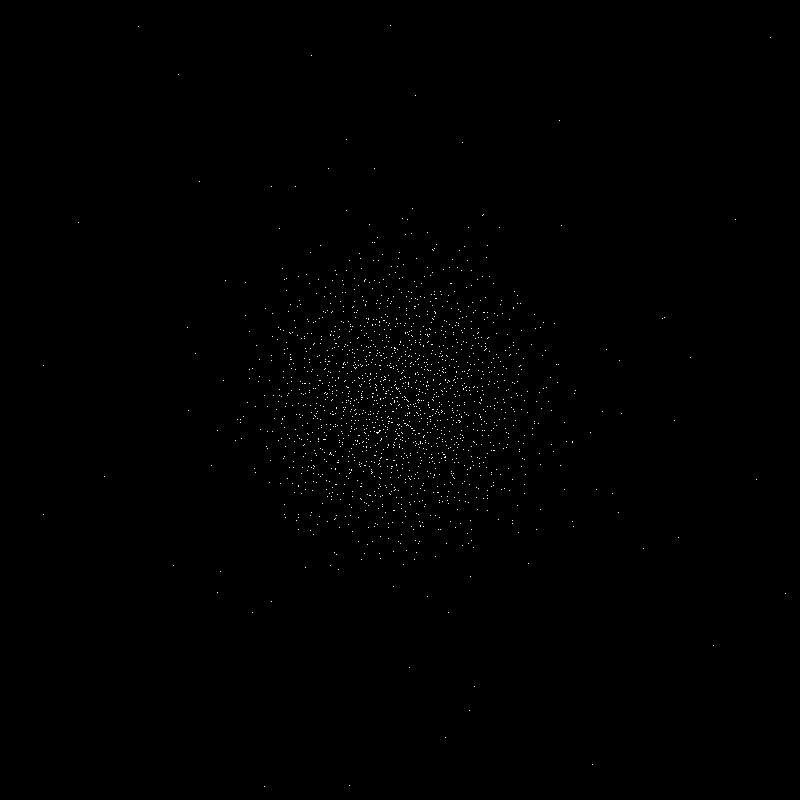
\includegraphics[width=0.9\linewidth]{reference_small}
    \caption{Year $\sim 250 \, 000$, at the peak of the first collapse.\\\ }
  \end{subfigure}
  \begin{subfigure}[b]{0.495\linewidth}
    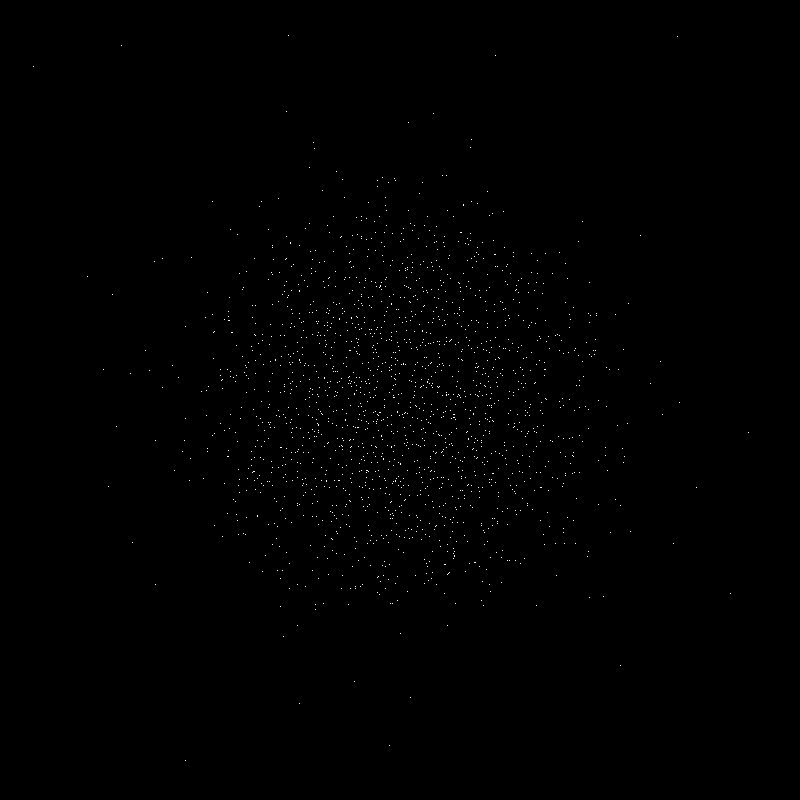
\includegraphics[width=0.9\linewidth]{reference_large}
    \caption{Year $\sim 550 \, 000$, just before the second collapse.}
  \end{subfigure}
  \caption{The reference simulation}
  \label{fig:coffee}
\end{figure}
\restoregeometry

\section{Very high initial temperature}

\subsection{Log}
\singlespacing
\begin{verbatim}
UPS Years    Move    Energy    Poten   Kinetic  Temp   Pressure
29       0  5.6e-12  1.23e37 -1.07e35  4.38e34 1000.00 9.2e-10
31   50000  5.0e-11  1.26e37 -3.59e34  3.70e36 723.06  6.6e-10
30  100000  6.6e-11  1.26e37 -1.96e34  3.76e36 716.80  6.6e-10
30  150000  9.9e-11  1.26e37 -1.35e34  3.77e36 715.97  6.6e-10
30  200000  3.0e-11  1.26e37 -1.02e34  3.77e36 715.75  6.6e-10
30  250000  9.4e-11  1.26e37 -8.26e33  3.77e36 715.67  6.6e-10
30  300000  9.4e-11  1.26e37 -6.93e33  3.77e36 715.63  6.6e-10
30  350000  5.0e-11  1.26e37 -5.96e33  3.77e36 715.61  6.6e-10
29  400000  1.2e-10  1.26e37 -5.24e33  3.76e36 715.60  6.6e-10
31  450000  1.3e-10  1.26e37 -4.67e33  3.76e36 715.60  6.6e-10
30  500000  6.7e-11  1.26e37 -4.21e33  3.76e36 715.59  6.6e-10
29  550000  9.8e-11  1.26e37 -3.83e33  3.76e36 715.59  6.6e-10
30  600000  1.3e-10  1.26e37 -3.52e33  3.76e36 715.59  6.6e-10
30  650000  1.2e-10  1.26e37 -3.25e33  3.76e36 715.58  6.6e-10
30  700000  1.2e-10  1.26e37 -3.02e33  3.76e36 715.58  6.6e-10
30  750000  1.3e-10  1.26e37 -2.82e33  3.76e36 715.58  6.6e-10
30  800000  5.5e-11  1.26e37 -2.65e33  3.76e36 715.58  6.6e-10
30  850000  5.5e-11  1.26e37 -2.49e33  3.76e36 715.58  6.6e-10
30  900000  6.9e-11  1.26e37 -2.36e33  3.76e36 715.58  6.6e-10
30  950000  1.1e-10  1.26e37 -2.23e33  3.76e36 715.58  6.6e-10
29 1000000  2.7e-10  1.26e37 -2.12e33  3.76e36 715.58  6.6e-10
29 1050000  9.9e-11  1.26e37 -2.02e33  3.76e36 715.58  6.6e-10
30 1100000  6.1e-11  1.26e37 -1.93e33  3.76e36 715.58  6.6e-10
30 1150000  6.3e-11  1.26e37 -1.85e33  3.76e36 715.58  6.6e-10
30 1200000  8.4e-11  1.26e37 -1.77e33  3.76e36 715.58  6.6e-10
30 1250000  1.8e-10  1.26e37 -1.70e33  3.76e36 715.58  6.6e-10
27 1300000  1.3e-10  1.26e37 -1.64e33  3.76e36 715.58  6.6e-10
30 1350000  1.6e-10  1.26e37 -1.58e33  3.76e36 715.58  6.6e-10
30 1400000  1.3e-10  1.26e37 -1.52e33  3.76e36 715.58  6.6e-10
30 1450000  7.5e-11  1.26e37 -1.47e33  3.76e36 715.58  6.6e-10
30 1500000  1.3e-10  1.26e37 -1.42e33  3.76e36 715.58  6.6e-10
30 1550000  1.4e-10  1.26e37 -1.37e33  3.76e36 715.58  6.6e-10
30 1600000  1.4e-10  1.26e37 -1.33e33  3.76e36 715.58  6.6e-10
30 1650000  1.2e-10  1.26e37 -1.29e33  3.76e36 715.58  6.6e-10
29 1700000  2.6e-10  1.26e37 -1.25e33  3.76e36 715.58  6.6e-10
30 1750000  1.8e-10  1.26e37 -1.22e33  3.76e36 715.58  6.6e-10
29 1800000  2.2e-10  1.26e37 -1.18e33  3.76e36 715.58  6.6e-10
30 1850000  3.1e-10  1.26e37 -1.15e33  3.76e36 715.58  6.6e-10
31 1900000  2.2e-10  1.26e37 -1.12e33  3.76e36 715.58  6.6e-10
30 1950000  2.5e-10  1.26e37 -1.09e33  3.76e36 715.58  6.6e-10
30 2000000  2.5e-10  1.26e37 -1.07e33  3.76e36 715.58  6.6e-10
\end{verbatim}
\onehalfspacing

\subsection{Comment}
The cloud starts rapidly expanding along the perimeter. Internal particles are first pushed inwards,
but start expanding outwards around year $100 \, 000$ when the outer particles no longer are present
to keep them inside. The expansion continues throughout the entire simulation.

\newgeometry{left=1.5cm,right=1.5cm}
\begin{figure}[p]
  \centering
  \begin{subfigure}[b]{0.495\linewidth}
    
\includegraphics[width=0.9\linewidth]{hot_start}
    \caption{Year $\sim 50 \, 000$, at the start of the rapid expansion.\\\ }
  \end{subfigure}
  \begin{subfigure}[b]{0.495\linewidth}
    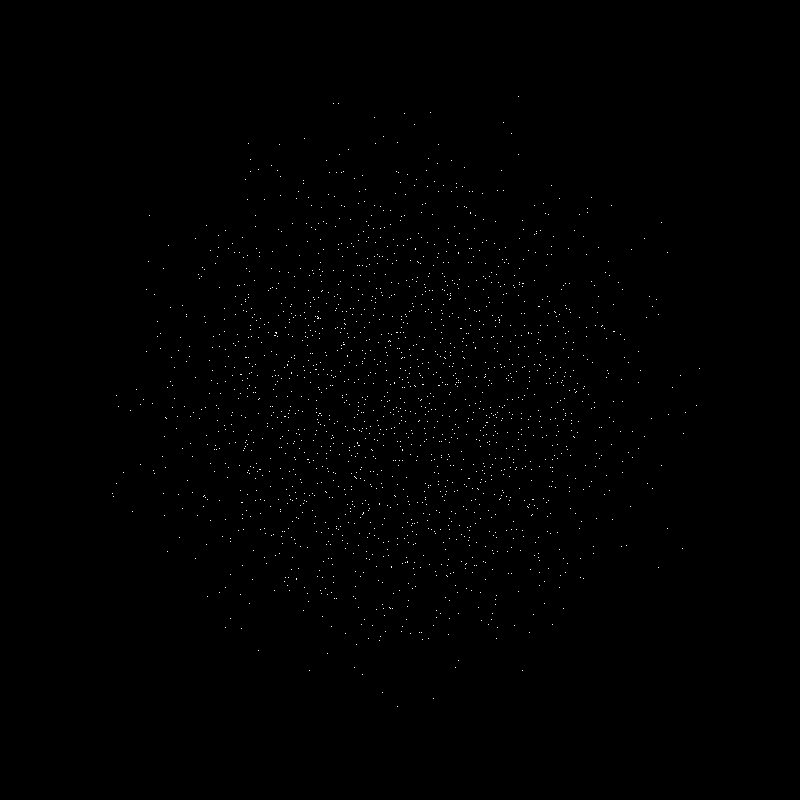
\includegraphics[width=0.9\linewidth]{hot_middle}
    \caption{Year $\sim 1 \, 000 \, 000$, zoomed out to make the entire cloud visible.\\\ }
  \end{subfigure}
  \begin{subfigure}[b]{0.495\linewidth}
    
\includegraphics[width=0.9\linewidth]{hot_end}
    \caption{Year $\sim 2 \, 000 \, 000$, at the same zoom level as the last picture. The cloud only
    just covers screen.
}
  \end{subfigure}
  \caption{The simulation with a very high initial temperature. Features such as a constellation
      remicient of the Big Dipper is visible in both $b$ and $c$ at 2 o'clock }
  \label{fig:coffee}
\end{figure}
\restoregeometry

\section{Rotating}

\subsection{Log}
\singlespacing
\begin{verbatim}
UPS Years    Move    Energy    Poten   Kinetic  Temp Pressure
29       0  5.9e-11  1.12e35 -1.07e35  1.56e35  5.00  4.6e-12
29   50000  4.1e-11  1.75e35 -9.63e34  2.16e35  4.42  4.0e-12
30  100000  1.6e-11  1.76e35 -7.98e34  2.06e35  4.05  3.7e-12
31  150000  2.7e-11  1.77e35 -6.67e34  1.95e35  3.90  3.6e-12
29  200000  2.9e-11  1.77e35 -5.71e34  1.86e35  3.82  3.5e-12
30  250000  9.9e-12  1.77e35 -4.99e34  1.80e35  3.79  3.5e-12
30  300000  2.4e-11  1.77e35 -4.42e34  1.74e35  3.78  3.5e-12
29  350000  2.0e-11  1.77e35 -3.94e34  1.70e35  3.75  3.4e-12
30  400000  3.9e-11  1.77e35 -3.54e34  1.67e35  3.72  3.4e-12
30  450000  2.1e-11  1.77e35 -3.19e34  1.63e35  3.69  3.4e-12
30  500000  2.5e-11  1.77e35 -2.90e34  1.61e35  3.67  3.4e-12
30  550000  3.5e-11  1.77e35 -2.65e34  1.58e35  3.66  3.3e-12
30  600000  1.6e-11  1.77e35 -2.44e34  1.56e35  3.65  3.3e-12
29  650000  1.2e-11  1.77e35 -2.26e34  1.55e35  3.64  3.3e-12
30  700000  1.5e-11  1.77e35 -2.11e34  1.53e35  3.64  3.3e-12
29  750000  3.5e-11  1.77e35 -1.98e34  1.52e35  3.63  3.3e-12
29  800000  1.1e-11  1.77e35 -1.86e34  1.51e35  3.63  3.3e-12
29  850000  4.3e-11  1.77e35 -1.75e34  1.50e35  3.63  3.3e-12
30  900000  2.3e-11  1.77e35 -1.66e34  1.49e35  3.63  3.3e-12
30  950000  3.2e-11  1.77e35 -1.58e34  1.48e35  3.63  3.3e-12
30 1000000  3.6e-11  1.77e35 -1.50e34  1.47e35  3.63  3.3e-12
30 1050000  4.0e-11  1.77e35 -1.44e34  1.47e35  3.63  3.3e-12
30 1100000  1.3e-11  1.77e35 -1.38e34  1.46e35  3.63  3.3e-12
30 1150000  2.1e-11  1.77e35 -1.32e34  1.46e35  3.63  3.3e-12
30 1200000  1.8e-11  1.77e35 -1.27e34  1.45e35  3.62  3.3e-12
30 1250000  3.0e-11  1.77e35 -1.22e34  1.45e35  3.62  3.3e-12
30 1300000  3.4e-11  1.77e35 -1.18e34  1.44e35  3.62  3.3e-12
30 1350000  2.8e-11  1.77e35 -1.14e34  1.44e35  3.62  3.3e-12
30 1400000  3.1e-11  1.77e35 -1.10e34  1.43e35  3.62  3.3e-12
30 1450000  1.6e-11  1.78e35 -1.06e34  1.44e35  3.62  3.3e-12
30 1500000  1.9e-11  1.78e35 -1.03e34  1.44e35  3.62  3.3e-12
30 1550000  3.5e-11  1.78e35 -9.97e33  1.44e35  3.62  3.3e-12
30 1600000  9.5e-12  1.78e35 -9.68e33  1.43e35  3.62  3.3e-12
30 1650000  2.0e-11  1.78e35 -9.44e33  1.43e35  3.62  3.3e-12
30 1700000  1.4e-11  1.78e35 -9.15e33  1.43e35  3.62  3.3e-12
31 1750000  3.9e-11  1.78e35 -8.91e33  1.43e35  3.62  3.3e-12
31 1800000  3.2e-11  1.78e35 -8.67e33  1.42e35  3.62  3.3e-12
30 1850000  5.3e-11  1.78e35 -8.45e33  1.42e35  3.62  3.3e-12
30 1900000  2.3e-11  1.78e35 -8.24e33  1.42e35  3.62  3.3e-12
30 1950000  2.8e-11  1.78e35 -8.05e33  1.42e35  3.62  3.3e-12
30 2000000  2.8e-11  1.78e35 -7.86e33  1.42e35  3.62  3.3e-12
\end{verbatim}
\onehalfspacing

\subsection{Comment}
The intial sphere is flattened to thin disk from year $0$ to $400 \, 000$. The disk then continues
to expand, taking a shape similar to a convex lens. After year $\sim 600 \, 000$, the shape no
longer deforms and instead expands uniformly.

\newgeometry{left=1.5cm,right=1.5cm}
\begin{figure}[p]
  \centering
  \begin{subfigure}[b]{0.495\linewidth}
    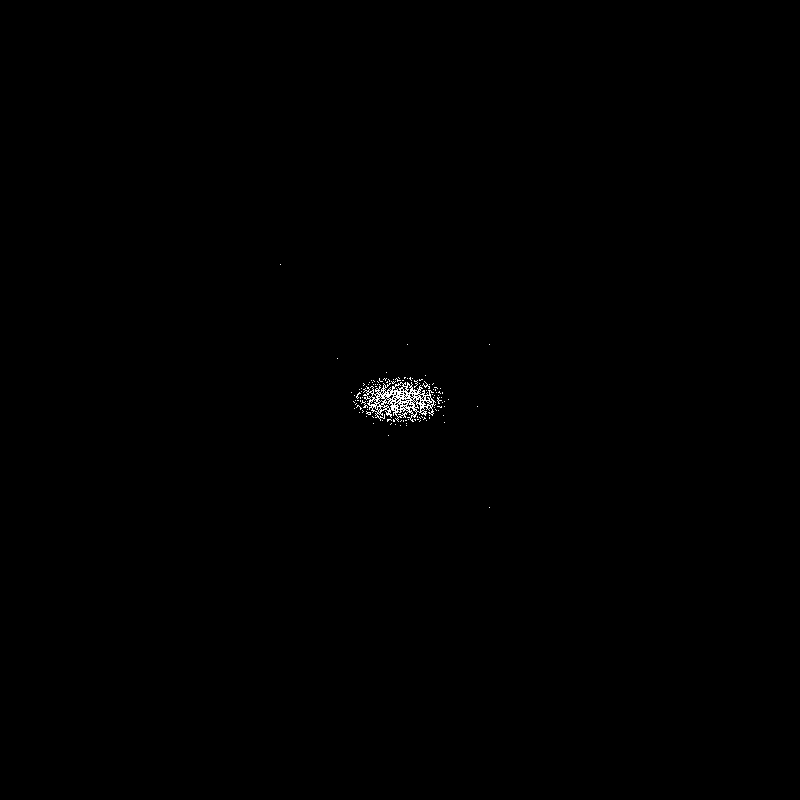
\includegraphics[width=0.9\linewidth]{rotating_start}
    \caption{Year $\sim 100 \, 000$, the sphere is starting to flatten.\\\ }
  \end{subfigure}
  \begin{subfigure}[b]{0.495\linewidth}
    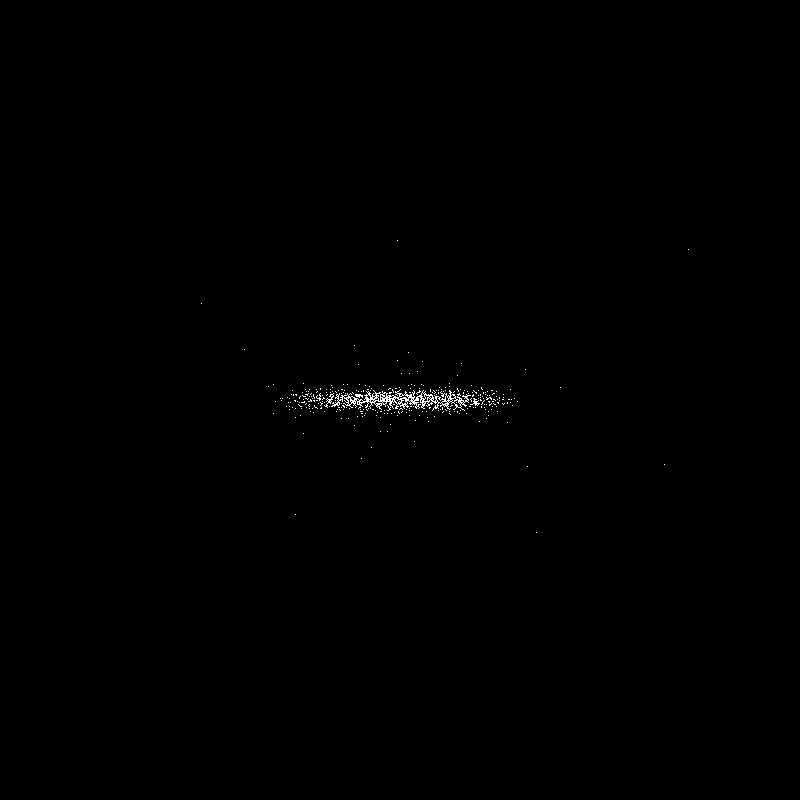
\includegraphics[width=0.9\linewidth]{rotating_flat}
    \caption{Year $\sim 400 \, 000$, the disk is at its thinnest point.\\\ }
  \end{subfigure}
  \begin{subfigure}[b]{0.495\linewidth}
    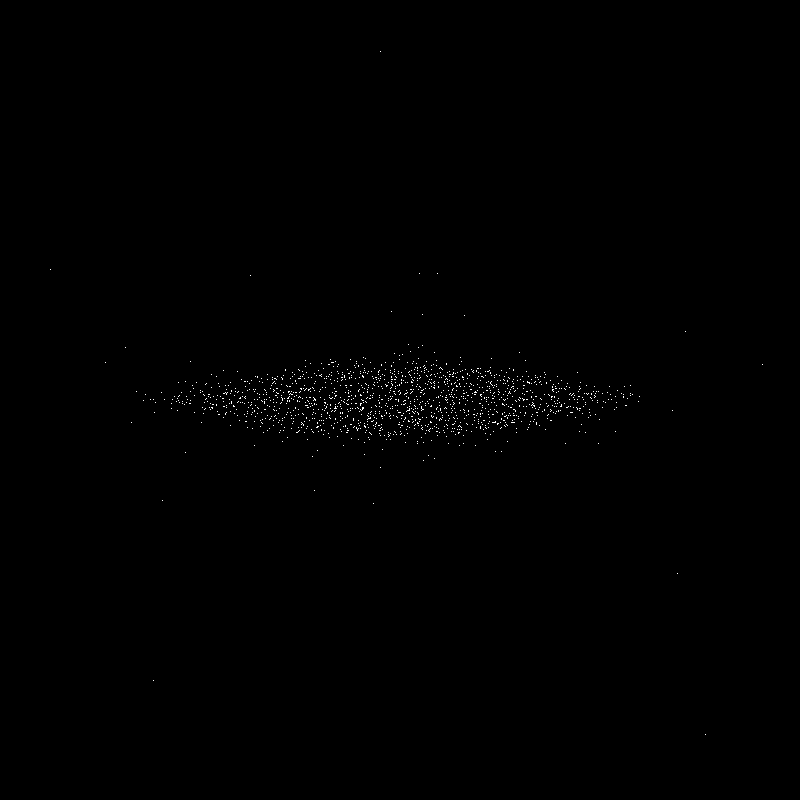
\includegraphics[width=0.9\linewidth]{rotating_eye}
    \caption{Year $\sim 900 \, 000$, the particles are expanding outwards. There is no noticable
    acceleration and as such the shape of a convex lens is maintained.}
  \end{subfigure}
  \caption{The rotating simulation without a dense core}
  \label{fig:coffee}
\end{figure}
\restoregeometry

\section{Rotating, with a dense core}

\subsection{Log}
\singlespacing
\begin{verbatim}
UPS Years    Move    Energy    Poten   Kinetic  Temp Pressure
29       0  1.5e-11 -3.02e34 -1.80e35  8.79e34  5.00  3.5e-10
30   50000  2.3e-10  5.68e36 -1.68e35  5.79e36  4.93  6.5e-11
30  100000  3.0e-10  5.68e36 -1.46e35  5.78e36  4.39  2.4e-11
28  150000  2.2e-10  5.69e36 -1.30e35  5.77e36  4.15  2.1e-11
30  200000  2.0e-10  5.69e36 -1.16e35  5.76e36  3.90  1.2e-11
30  250000  2.0e-10  5.69e36 -1.05e35  5.75e36  3.68  1.0e-11
30  300000  1.8e-10  5.69e36 -9.72e34  5.75e36  3.48  9.3e-12
29  350000  2.5e-10  5.70e36 -9.13e34  5.74e36  3.38  8.0e-12
30  400000  2.3e-10  5.70e36 -8.67e34  5.74e36  3.33  6.7e-12
30  450000  2.3e-10  5.70e36 -8.50e34  5.74e36  3.38  7.0e-12
30  500000  2.1e-10  5.70e36 -8.46e34  5.74e36  3.43  7.3e-12
30  550000  2.3e-10  5.70e36 -8.48e34  5.74e36  3.47  8.3e-12
29  600000  2.2e-10  5.70e36 -8.34e34  5.74e36  3.46  6.9e-12
29  650000  1.9e-10  5.70e36 -8.17e34  5.74e36  3.43  6.5e-12
30  700000  2.4e-10  5.72e36 -7.99e34  5.76e36  3.38  6.1e-12
30  750000  2.0e-10  5.72e36 -7.78e34  5.75e36  3.33  5.4e-12
30  800000  2.6e-10  5.72e36 -7.60e34  5.75e36  3.30  5.2e-12
30  850000  3.0e-10  5.72e36 -7.47e34  5.75e36  3.26  4.7e-12
30  900000  2.9e-10  5.73e36 -7.38e34  5.76e36  3.27  4.9e-12
30  950000  3.7e-10  5.73e36 -7.28e34  5.76e36  3.27  4.8e-12
28 1000000  2.7e-10  5.73e36 -7.18e34  5.77e36  3.24  4.3e-12
30 1050000  2.7e-10  5.73e36 -7.15e34  5.77e36  3.25  4.7e-12
29 1100000  2.5e-10  5.74e36 -7.03e34  5.77e36  3.21  4.2e-12
30 1150000  3.1e-10  5.74e36 -6.95e34  5.77e36  3.20  4.2e-12
28 1200000  2.2e-10  5.74e36 -6.90e34  5.77e36  3.20  4.2e-12
30 1250000  2.4e-10  5.74e36 -6.82e34  5.77e36  3.16  4.1e-12
31 1300000  3.0e-10  5.74e36 -6.72e34  5.77e36  3.14  4.1e-12
30 1350000  1.8e-10  5.74e36 -6.61e34  5.77e36  3.13  3.9e-12
30 1400000  2.3e-10  5.74e36 -6.50e34  5.77e36  3.12  3.7e-12
30 1450000  2.7e-10  5.74e36 -6.38e34  5.77e36  3.11  3.5e-12
31 1500000  1.5e-10  5.74e36 -6.29e34  5.77e36  3.09  3.5e-12
30 1550000  2.5e-10  5.74e36 -6.20e34  5.77e36  3.08  3.4e-12
30 1600000  2.1e-10  5.74e36 -6.11e34  5.77e36  3.08  3.4e-12
30 1650000  1.7e-10  5.75e36 -6.03e34  5.77e36  3.07  3.3e-12
29 1700000  2.4e-10  5.75e36 -5.95e34  5.77e36  3.05  3.2e-12
30 1750000  2.6e-10  5.75e36 -5.89e34  5.77e36  3.04  3.2e-12
30 1800000  2.6e-10  5.75e36 -5.85e34  5.77e36  3.02  3.1e-12
31 1850000  2.5e-10  5.75e36 -5.82e34  5.77e36  3.02  3.2e-12
31 1900000  2.8e-10  5.75e36 -5.76e34  5.77e36  3.01  3.1e-12
31 1950000  1.8e-10  5.75e36 -5.70e34  5.77e36  3.01  3.0e-12
31 2000000  2.1e-10  5.75e36 -5.65e34  5.77e36  3.00  3.0e-12
\end{verbatim}
\onehalfspacing

\subsection{Comment}
The initial sphere flattens from year $0$ to $300 \, 000$. The outer envelope then expands, taking
on the shape of a convex lens. The core maintains its mass and size throughout the simulation. At
year $1 \, 200 \, 000$ the core visible rotates with a period similar to the initial rotational
period.

\newgeometry{left=1.5cm,right=1.5cm}
\begin{figure}[p]
  \centering
  \begin{subfigure}[b]{0.495\linewidth}
    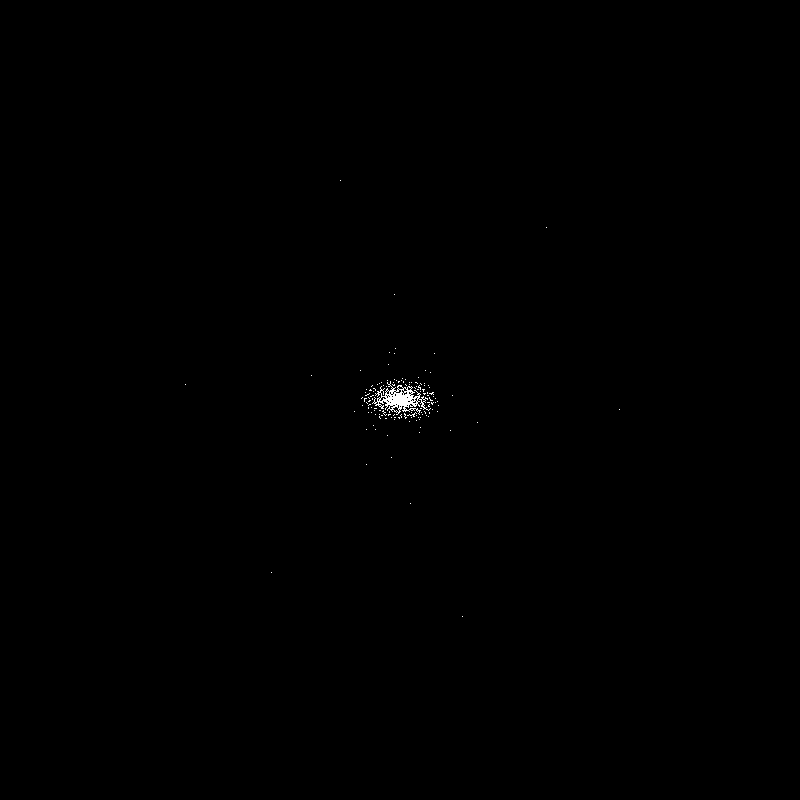
\includegraphics[width=0.9\linewidth]{core_start}
    \caption{Year $\sim 100 \, 000$. The initial sphere is flattening and the \\ dense core is clearly
    visible.\\\ }
  \end{subfigure}
  \begin{subfigure}[b]{0.495\linewidth}
    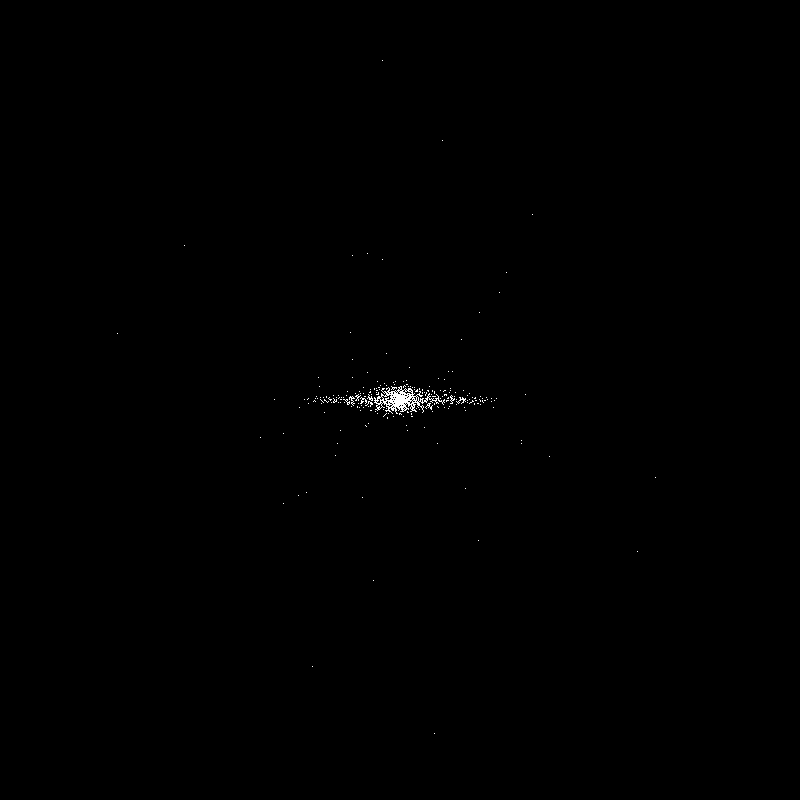
\includegraphics[width=0.9\linewidth]{core_galaxy}
    \caption{Year $\sim 300 \, 000$. The disk is at its flattest point, bulging \\ due to the dense and
    relatively spherical core.\\\ }
  \end{subfigure}
  \begin{subfigure}[b]{0.495\linewidth}
    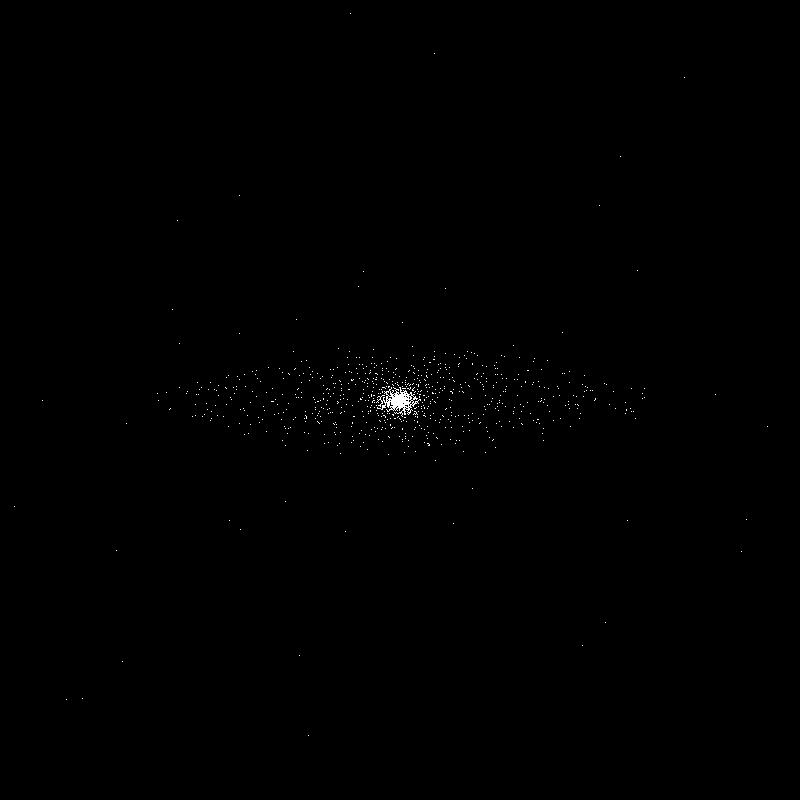
\includegraphics[width=0.9\linewidth]{core_eye}
    \caption{Year $\sim 1 \, 000 \, 000$. The outer particles expand uniformly \\ while the core
    maintains its particles.}
  \end{subfigure}
  \begin{subfigure}[b]{0.495\linewidth}
    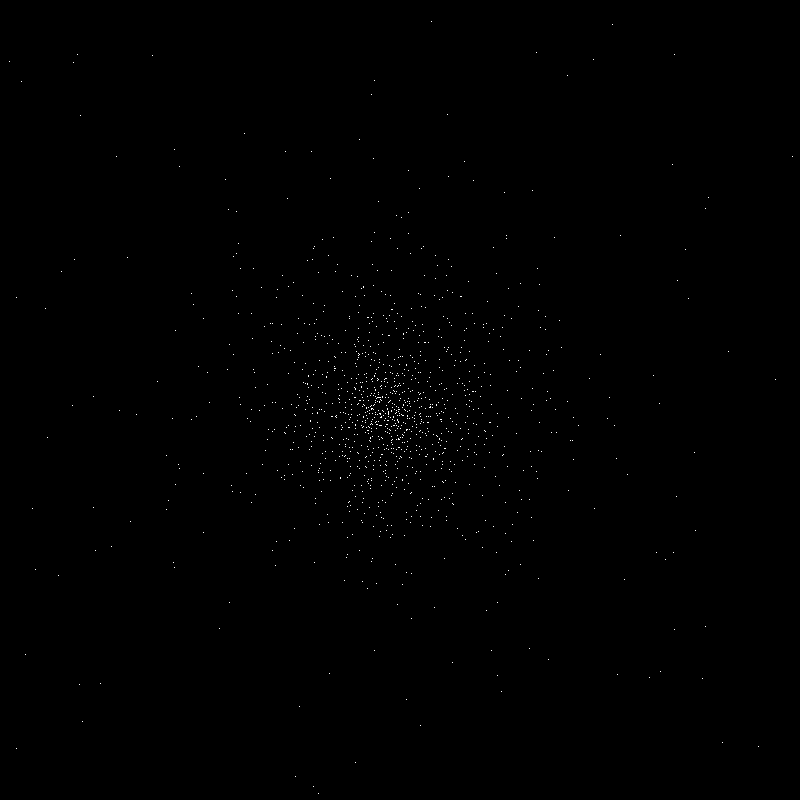
\includegraphics[width=0.9\linewidth]{core_core}
    \caption{Year $\sim 1 \, 200 \, 000$, zoomed on the core from above the \\ rotational plane.}
  \end{subfigure}
  \caption{The rotating simulation with a dense core}
  \label{fig:coffee}
\end{figure}
\restoregeometry

\end{document}
